\chapter{Apache Hadoop}
In this chapter, I will briefly introduce the technologies I worked with. To understand the memory issues and their proposed resolution, a high level overview of the technology stack is needed.

Apache Hadoop is an open source distributed framework for managing, processing and storing large amounts of data in clustered systems built from commodity hardware. All modules in Hadoop were designed with an assumption that hardware failures are frequent and should be automatically handled by the framework. One of the most important characteristics of Hadoop is that it partitions data and computation across many hosts and executes computation in parallel close to the data it uses.  \cite{Hadoop-wiki}

\noindent The base of the Hadoop framework contains the following modules:
\begin{itemize}
	\item HDFS - Hadoop Distributed File System: designed to store large data sets reliably and stream those at high bandwidth to user applications
	\item Hadoop MapReduce: an implementation of the MapReduce programming model for large data processing
	\item YARN - Yet Another Resource Negotiator: a resource management and job scheduling technology
	\item Hadoop Common: contains libraries and utilities for other Hadoop modules
\end{itemize}

\section{HDFS - Hadoop Distributed File System}
HDFS is the file system of Hadoop. It stores file system metadata and application data separately. The dedicated server that stores metadata is the NameNode. Application data is stored on other servers called DataNodes. These servers are connected and they communicate using TCP-based protocols \cite{Shvachko:2010:HDF:1913798.1914427}. 

\noindent The file system is based on the following goals and principles \cite{Hadoop-current}:
\begin{itemize}
	\item \textbf{Hardware failure}: Hardware failures should be considered as normal, rather than an exception. An HDFS instance consists hundreds or thousands of components so this means that some of them will always be non-functional. Therefore, fault detection and automatic recovery is a must.
	\item \textbf{Streaming Data Access}: HDFS was designed for batch processing rather than interactive use. Therefore, HDFS users need streaming access to their data. This means that high throughput is more important than low latency.
	\item \textbf{Large Data Sets}: The size of a typical HDFS file is gigabytes to terabytes. Thus, the file system is tuned to support large files. 
	\item \textbf{Simple Coherency}: HDFS follows the WORM (Write-Once-Read-Many) model. A file, once written, should not be changed except for appends and truncates.  This assumption simplifies data coherency issues. A MapReduce application fits perfectly for this model.
	\item \textbf{Moving computation}: A computation is much more efficient if it is executed near the data it operates on. This is especially true for big data. 
	\item \textbf{Portability}: HDFS was designed to port from one platform to another with ease. 
\end{itemize}

\subsection{NameNode}
NameNode keeps the directory tree of all files in the file system and tracks where data is kept across the cluster; it does not store the files. Clients talk to the NameNode whenever they want to locate a file. The NameNode's response is a list of relevant DataNode servers where the data is available. 

As a result of this approach, NameNode is a Single Point of Failure in the HDFS cluster. Whenever the NameNode goes down, the file system becomes unavailable.
\begin{figure}[H]
	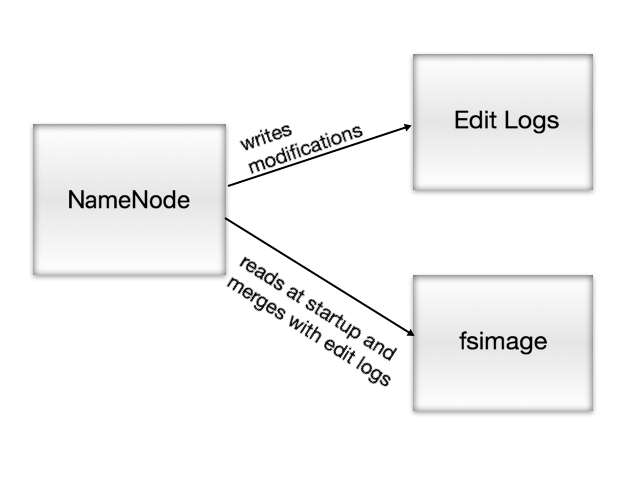
\includegraphics[width=80mm, keepaspectratio]{figures/namenode_problem.png}
	\centering
	\caption{Problem with NameNode}
\end{figure}
The image shows how NameNode stores information \cite{Secondary-NameNode}. There are two different files:
\begin{itemize}
	\item edit logs: the changes made to the file system after the NameNode started
	\item fsimage: a snapshot of the file system when the NameNode started
\end{itemize}
In production clusters, the NameNode restarts are very rare. That means edit logs can grow large and in case of a crash we will lose a huge amount of metadata since the fsimage is very old.

The Secondary NameNode helps to solve this issue. It is responsible for merging the edit logs with fsimage. It collects edit logs on a regular basis and applies them to the fsimage. NameNode will use this fsimage in case of a crash and it can also be used to reduce the startup time of the NameNode.
It is important to remember that the Secondary NameNode is not a real backup NameNode, it only merges the edits into the fsimage. 

\begin{figure}[H]
	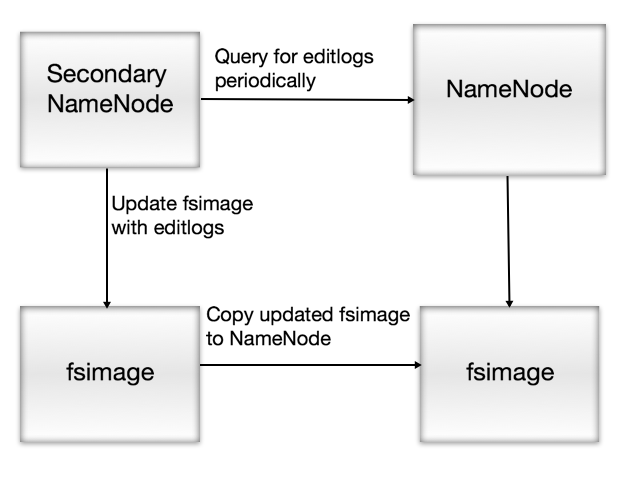
\includegraphics[width=80mm, keepaspectratio]{figures/secondary_namenode.png}
	\centering
	\caption{Solution using the Secondary NameNode}
\end{figure}

\subsection{DataNodes \cite{Shvachko:2010:HDF:1913798.1914427}}
On a DataNode, a block is represented by two files in the native file system. The first contains the data itself, the second is the metadata.

On startup, the DataNodes connect to the NameNode and perform a handshake. This will verify the namespace ID and software version of the DataNodes. If one of them does not match the NameNode's value, the DataNode automatically shuts down. After a successful handshake, the DataNode registers with the NameNode. The DataNode will store its internal identifier. If a restart occurs, the DataNodes will be recognizable with the ID, even if they get a different IP address or port. After the ID is registered to the NameNode, it will never change. 

 When a DataNode is registered, it sends a block report immediately. It contains a block ID, generation stamp and the length of each block the DataNode hosts. To provide up-to-date information to the NameNode, reports are sent every hour. 

DataNodes send heartbeats to the NameNode. This ensures the NameNode that the DataNode is operating and block replicas of the server are available. If the NameNode does not receive a heartbeat from a DataNode it will consider the node to be out of service. The default heartbeat interval is three seconds.

\subsection{HDFS Client \cite{Shvachko:2010:HDF:1913798.1914427}}
User applications can access the file system using the HDFS client which exports the HDFS file system interface. HDFS supports operations similar to a traditional file system: read, write, create or delete files and create or delete directories. The user can refer to files or directories using paths in the namespace.

When someone reads a file, the HDFS client asks the NameNode for the list of DataNodes that host replicas of the blocks of the file. Then it will directly contact the DataNode and request the desired block.

\begin{figure}[H]
	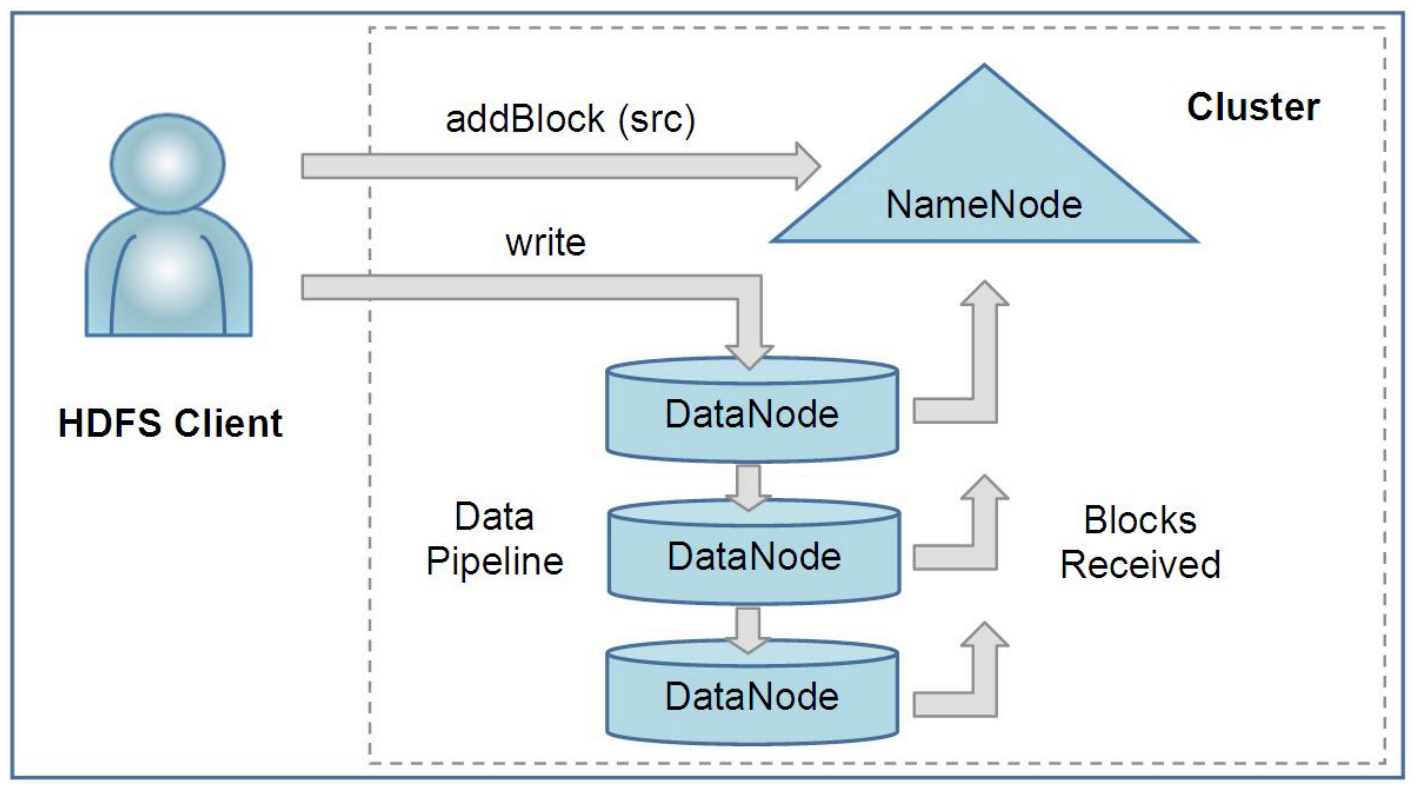
\includegraphics[width=100mm, keepaspectratio]{figures/hdfs_client.png}
	\centering
	\caption{HDFS file writing  \cite{Shvachko:2010:HDF:1913798.1914427}}
\end{figure}
The client creates a new file by giving its path to the NameNode. For each block, the NameNode will return a list of DataNodes to place the replicas. The client pipelines data to the given DataNodes, and they will confirm the creation of the block to the NameNode.

\section{MapReduce}
MapReduce is a programming model for processing data sets. Users specify two functions \cite{Dean:2004:MSD:1251254.1251264}:
\begin{itemize}
	\item map function: processes a key-value pair to generate a set of key-value pairs
	\item reduce function: merges the intermediate values associated with the same key
\end{itemize}

Programs written in MapReduce are automatically executed parallelly on large clusters. Using this, programmers with no experience in parallel programming and distributed systems can utilize the available resources on the cluster.
\paragraph{Example \cite{MapReduce-example} \label{example}}
This example shows how MapReduce handles the problem of counting words. Let's say we have the following list of words: 
\begin{center}
	\textbf{Dear, Bear, River, Car, Car, River, Deer, Car, Bear}
\end{center}

\begin{figure}[H]
	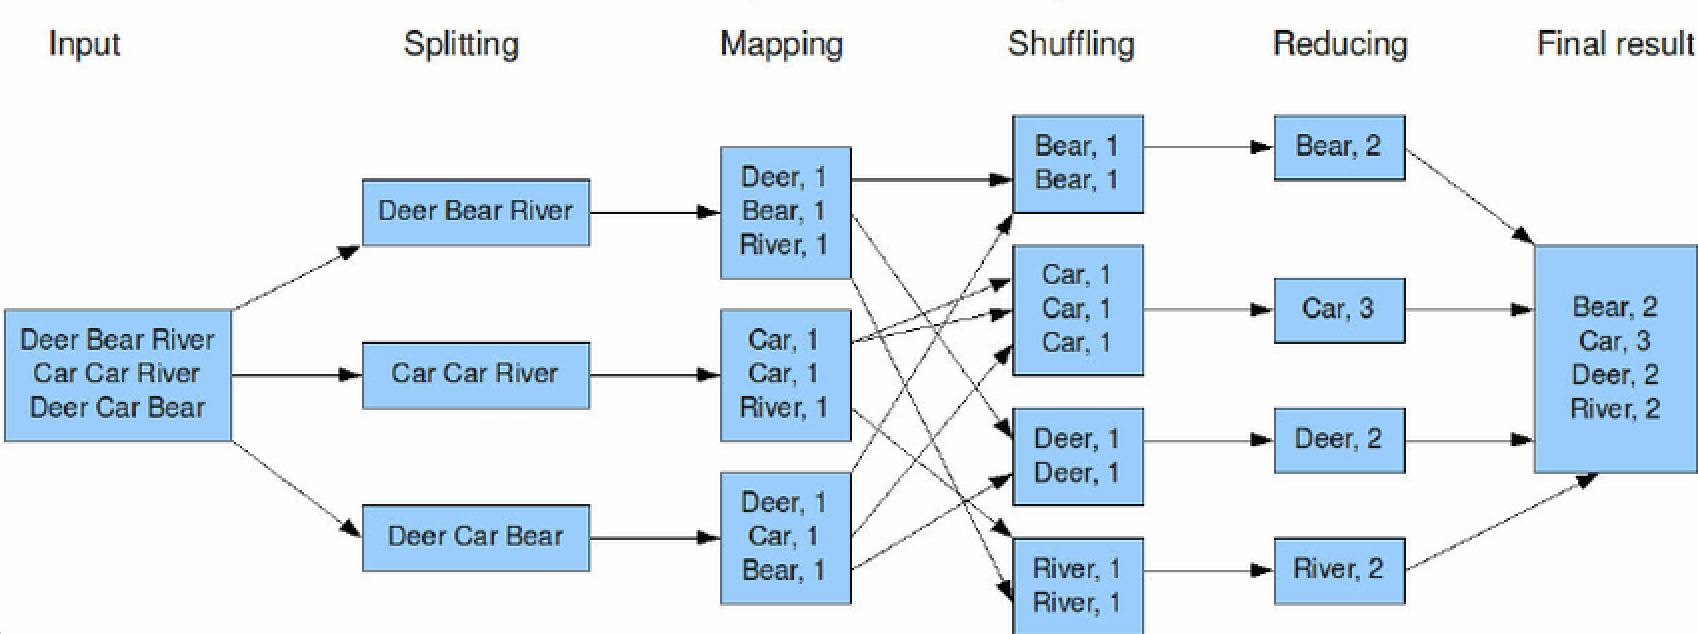
\includegraphics[width=150mm, keepaspectratio]{figures/MapReduce_Example.png}
	\caption{The MapReduce word count process \cite{MapReduce-example-figure}}
	\centering
\end{figure}
\begin{itemize}
	\item \textbf{Splitting}: the first step is dividing the input into splits. This will distribute the work among the Map nodes.
	\item \textbf{Mapping}: tokenize the words in each mapper and give a value of 1 for each word, since every word in itself will occur once.
	\item \textbf{Shuffling}: partition takes place with shuffling and sorting: this way, pairs with the same key will be sent to the same reducer.
	\item \textbf{Reducing}: a reducer gets the list of pairs and counts the number of ones in this list.
\end{itemize}

\subsection{Advantages of MapReduce \cite{MapReduce-example}}
\subsubsection{Parallel processing}
In MapReduce we divide the job among multiple nodes, so they can work on their part of the data parallelly. This way, data processing is done by multiple machines instead of one, so the time is significantly reduced.
\subsubsection{Data locality}
In Hadoop MapReduce, instead of moving data into the processing unit, we move the processing unit to the data. The traditional approach has its limit when it comes to processing big data. Moving large amounts of data is costly: network issues can occur and the master node (where data is stored) can get overloaded and may fail. 

However, the MapReduce approach is very cost efficient, since all the nodes are working simultaneously on their part of the data and there is no chance of a node getting overloaded.

Using Hadoop we just need to provide the map and reduce functions, the rest is done by the framework.  The word count example (\ref{example}) would look like the following in Java:
\subsubsection*{Map  \cite{MapReduce-example}}
\begin{lstlisting}[language=Java]
	public void map(LongWritable key, Text value, Context context) throws IOException,InterruptedException {
		String line = value.toString();
		StringTokenizer tokenizer = new StringTokenizer(line);
		while (tokenizer.hasMoreTokens()) {
			value.set(tokenizer.nextToken());
			context.write(value, new IntWritable(1));
		}
	}
\end{lstlisting}
The input and output of the Mapper is a key/value pair. 

\noindent Input:
\begin{itemize}
	\item Key: the offset of each line
	\item Value: each line
\end{itemize}

\noindent Output:
\begin{itemize}
	\item Key: the tokenized words
	\item Value: the hardcoded value 1
\end{itemize}

\subsubsection*{Reduce  \cite{MapReduce-example}}
\begin{lstlisting}
	public void reduce(Text key, Iterable<IntWritable> values,Context context) throws IOException,InterruptedException {
		int sum=0;
		for(IntWritable x: values) {
			sum+=x.get();
		}
		context.write(key, new IntWritable(sum));
	}
\end{lstlisting}
Both the input and output of the Reducer is a key/value pair. 

\noindent Input:
\begin{itemize}
	\item Key: unique words, generated after the sorting and shuffling phase
	\item Value: a list of integers corresponding to each keys
	\item \eg Bear, [1, 1]
\end{itemize}

\noindent Output:
\begin{itemize}
	\item Key: all the unique words in the input text file
	\item Value: number of occurrences for each unique word
	\item \eg  Bear, 2; Car, 3
\end{itemize}

The traditional way to execute MapReduce operations is that the users specify the Map and Reduce functions in Java. However, this approach has some problems:
\begin{itemize}
	\item it is not a high-level language for data processing
	\item data scientists do not understand Java. They came from the world of traditional databases, where SQL is used.
	\item even a simple problem can result in hundreds of lines of code.
\end{itemize}

Although, the Hadoop MapReduce framework is written in Java, with the help of Streaming API we can create Map and Reduce functions in any language.

MapReduce gives us a solution for many big data problems. However, for some scenarios, MapReduce is not the ideal choice: \eg real-time analysis. In Hadoop 1.0 we could not use components other than MapReduce (like Apache Storm which is ideal for real-time computation). The desire for utilizing the potential provided by the distributed file system (HDFS) for other solutions grew. YARN was the answer to fulfill this claim.

\section{YARN  \cite{Hadoop-current}}
\subsection{Hadoop 1.0 resource management}
Previous to Hadoop 2.0, a single JobTracker was responsible for monitoring resources, distributing MapReduce jobs for the DataNodes and monitoring these jobs. 

In Hadoop 1.0 the MapReduce module was responsible for cluster resource management and data processing as well.

\begin{figure}[H]
	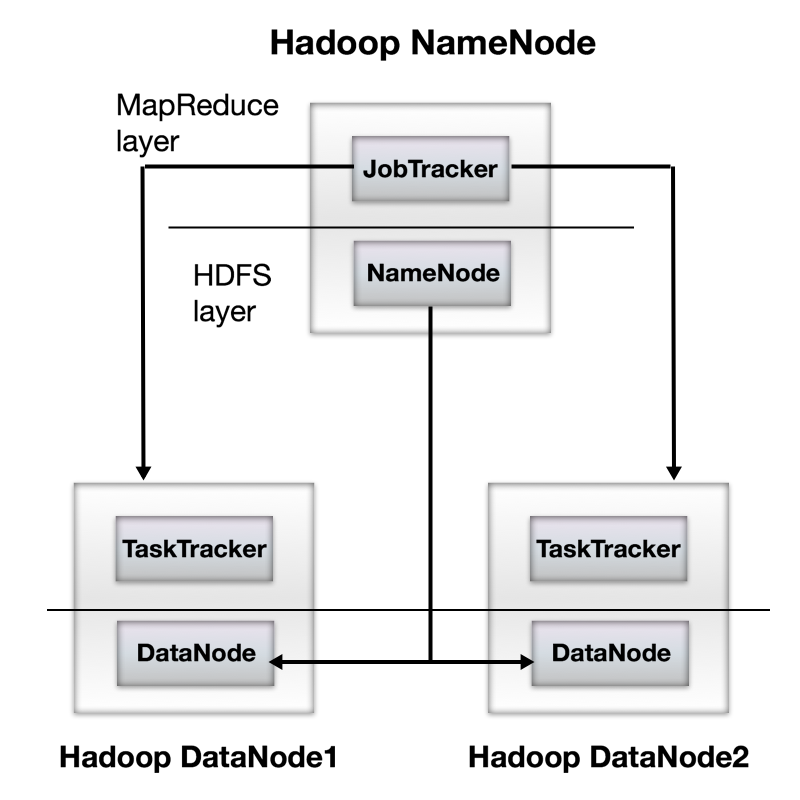
\includegraphics[width=100mm, keepaspectratio]{figures/hadoop10.png}
	\centering
	\caption{Hadoop 1.0 architecture \cite{Hadoop1.0-problems}}
	\centering
\end{figure}

\iffalse\noindent Resource management in Hadoop 1.0 \cite{Hadoop1.0}:

Clients submit jobs to the JobTracker which turns to the NameNode. It returns the location of the data. The JobTracker locates TaskTracker nodes with available slots close to the data and sends the job to the chosen TaskTracker nodes. After the job has started, the JobTracker monitors the chosen TaskTracker nodes. If they do not send heartbeats frequently, they are deemed to have failed, so the task will be scheduled on a different TaskTracker. The JobTracker gets a notification if a task fails. It decides what to do then: it may send the job to another TaskTracker, it can mark the record as something to avoid, or it may even put the TaskTracker to blacklist since it is unreliable. If the JobTracker sees that the task is finished, it will update its status. Clients poll the JobTracker for information.

\noindent The architecture of Hadoop 1.0 has many problems \cite{Hadoop1.0-problems}:
\begin{itemize}
	\item  It \textbf{limits scalability} since the JobTracker runs on a single machine doing multiple tasks, it becomes a bottleneck: resource management, job and task scheduling, and monitoring are done by the JobTracker.
	\item JobTracker is a \textbf{Single Point of Failure}. If it goes down, all the jobs are halted.
	\item In Hadoop 1.0, \textbf{JobTracker is tightly integrated with the MapReduce} module so only MapReduce applications can run on Hadoop. Although MapReduce is powerful enough to express many data analysis algorithms (mostly batch-driven data analysis), it is not always the optimal paradigm. It is often desirable to run other computation paradigms on Hadoop, like real-time analysis and Message-Passing approach, \etc. Since HDFS makes it easy to store large amounts of data it is desirable to utilize this for other big data problems.
\end{itemize}

Developers recognized that splitting the responsibility to resource management and application monitoring has serious benefits. YARN is a re-architecture of Hadoop that allows multiple applications to run on the same platform. With YARN, applications run "in" Hadoop, instead of "on" Hadoop. This takes Hadoop beyond a batch processing application to a "data operating system" where HDFS is the file system and YARN is the operating system. 

\begin{figure}[H]
	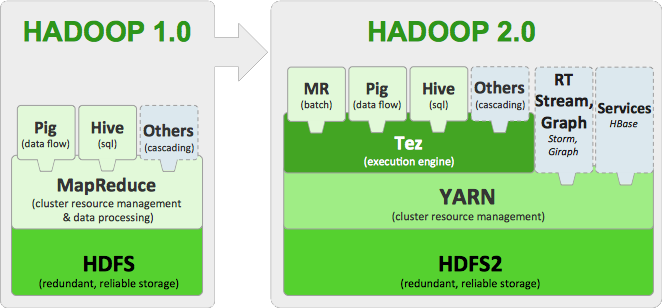
\includegraphics[width=100mm, keepaspectratio]{figures/hadoop10vs20.png}
	\centering
	\caption{From Hadoop 1.0 to Hadoop 2.0}
	\centering
\end{figure}
\fi
The fundamental idea behind YARN is to split up the functionalities of resource management and job scheduling/monitoring. In YARN we have a global ResourceManager (RM) and ApplicationMaster (AM) for each application.

\textbf{ResourceManager} is responsible for distributing the resources among all the applications in the system. The \textbf{NodeManager} is a per-machine agent who monitors the resource usages (CPU, memory, network, disk) of the containers and reports them to the ResourceManager. 

The \textbf{ApplicationMaster} is framework-specific, and its task is to ask the ResourceManager for resources when needed. It is also working with the NodeManagers to execute and monitor tasks.

The ResourceManager is divided into two main components: Scheduler and ApplicationsManager.
\begin{itemize}
	\item The Scheduler is responsible for allocating resources to applications running in the cluster. It schedules based on the resource requirements of each application. The Scheduler does not perform monitoring or status tracking.
	\item The ApplicationsManager accepts job submissions. It negotiates the first container for executing the application-specific ApplicationMaster. It is also responsible for restarting the ApplicationMaster if it fails. 
\end{itemize}

\begin{figure}[H]
	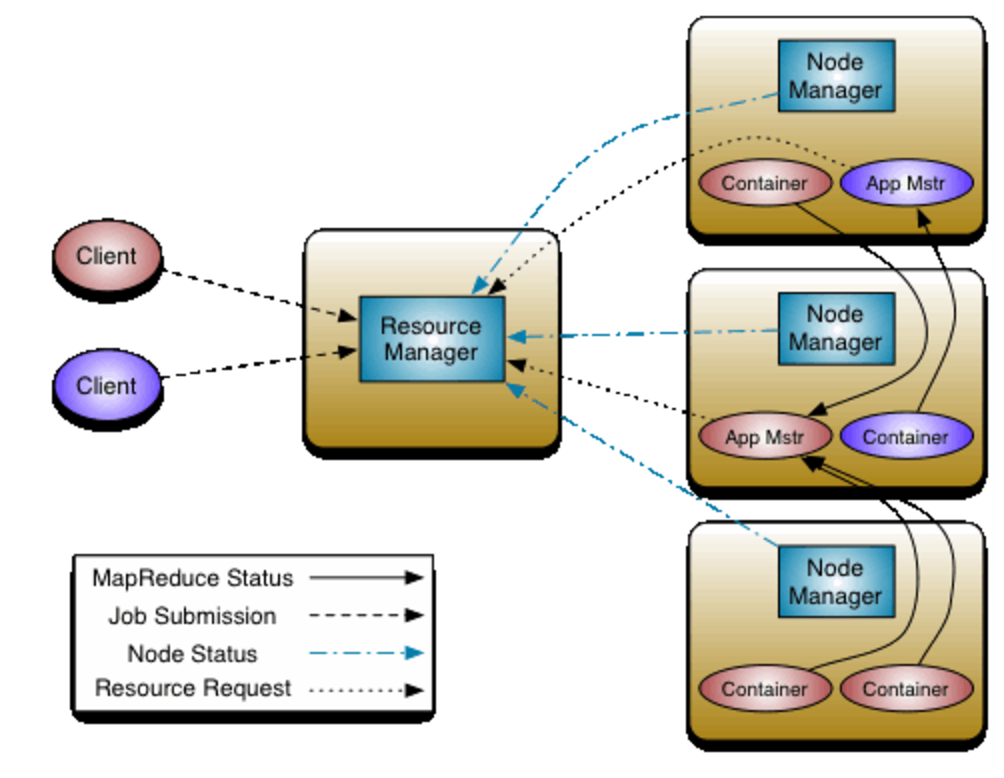
\includegraphics[width=110mm, keepaspectratio]{figures/yarn.png}
	\centering
	\caption{Yarn architecture}
	\centering
\end{figure}

In summary, with YARN Hadoop is able to run applications that do not follow the MapReduce model since it decouples the resource management and scheduling capabilities of MapReduce. With the help of YARN, we can efficiently utilize the resources and can run multiple applications in Hadoop, all sharing common resources.